\chapter{Matching Spatial and Temporal Boundary Conditions in Low-$k$ Modes}\label{chapter:low-k}

\chapterabstract{
% Editor's note: Rewrote the abstract for clarity, flow, and conciseness.
In conformal time, the age of the universe becomes finite, and solutions to the Friedmann equations and cosmological perturbations exhibit periodicity. This temporal periodicity imposes boundary conditions that restrict allowed wave vectors to discrete values, which are generally inconsistent with those required by the spatial boundary conditions of a closed universe. This chapter identifies general linear combination solutions that simultaneously satisfy both spatial and temporal boundary conditions. The resulting mode mixing and omissions yield a primordial power spectrum (PPS) and a cosmic microwave background (CMB) power spectrum characterized by suppression and fluctuations at low $k$. These theoretical features have the potential to explain observed anomalies in \texttt{Planck} data.
}


% Introduction: perturbations in periodic universe -> discrete wave vectors -> low-k mode -> 1975 paper solution -> structure of the paper 

% 1. Mathematical Method, describe topological picture
% 2. Toy model, shows it works 
% 3. Cosmology 
% 4. Future work

\section{Introduction}

% Editor's note: Improved the flow of the opening paragraph. Rephrased awkward constructs like "till (physical) time goes to infinity" and "co-expand".

In \cref{chapter:theory}, we pointed out that the two distinct sets of discrete wave vectors--coming from temporal and spatial periodic BCs respectively--must be consistent with each other, providing a strong constraint on cosmological parameters. To facilitate comparisons with observations, we solved the perturbations numerically and derived precise constraint values for these parameters by comparing with \texttt{Planck 2018} data (in \cref{chapter:Observation}).

However, a hidden complexity remains in this framework. The two sets of discrete wave vectors can be matched because they are both equally spaced in the high-$k$ regime. The wave vectors derived from the spatial BC are equally spaced by definition ($\propto n\in\mathbb{N}$). In contrast, for the temporal BC, the discrete $k$ values become non-equally spaced in the low-$k$ regime, as the frequencies become sufficiently low that the effects of the finite temporal boundary condition can no longer be ignored. 

The goal of this chapter is to find \textbf{general} solutions that satisfy both sets of BCs simultaneously. We demonstrate that these solutions must be linear combinations of the basis functions corresponding to each individual BC. The coefficients for these linear combinations are determined by the eigenvectors of projection matrices, which are computed via the inner products of the two sets of basis functions. The structure of the chapter is as follows: First, we define the problem in \cref{sec:def_PDE}, explain the mathematical and geometric interpretation of our method in \cref{sec:linear_combine_solution}, and demonstrate its efficacy using a 2D toy model in \cref{sec:toy_model}. We then apply this methodology to cosmological perturbations in \cref{sec:real_cosmology_lowk}, and generate the primordial power spectrum (PPS) and cosmic microwave background (CMB) power spectrum from these solutions in \cref{sec:PPS_CMB}. Finally, we outline potential applications and avenues for future work in \cref{sec:future_work}. 

\section{Problem Formulation}\label{sec:def_PDE}

% Structure:
% 1. Define the PDE and its periodic BCs. 
% 2. Solve eigenvalue problem -> solution with discrete wave vectors. 
% 3. The bases with different BCs are miss-match -> change T or L to match them in high-k mode
% 4. If $m\neq 0$, miss-match in low-k modes.

Our original goal was to solve the perturbation equations within a closed, periodic universe. This problem can be intuitively simplified into a 2D toy model: standing waves $\Phi$ in a 1D cavity, which evolve periodically. In other words, the waves must be periodic in both the spatial and temporal directions. The solution is trivial for a massless field, $\partial_t^2\Phi - \partial_x^2\Phi=0$, which yields simple plane waves (see \cref{fig:plane_waves_x-t_contour}).

\begin{figure}
    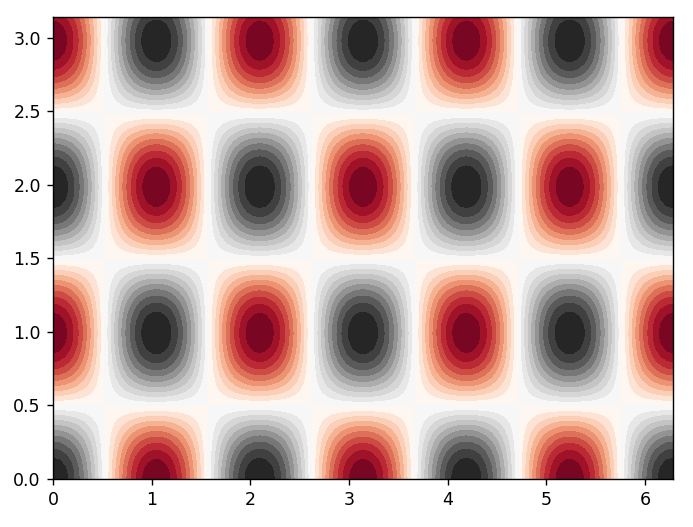
\includegraphics[width=0.5\textwidth]{parts/part1/figures/plane_waves_x-t_contour.png}
    \centering
    \caption{Contour plot of the plane wave $\Phi(x,t)=\exp(ikx)\cos(\omega t)$ in the $x-t$ plane, with wave vector $k=3$. The wave is periodic along both the $x$-axis and the $t$-axis.}
    \label{fig:plane_waves_x-t_contour}
\end{figure}

However, when generalized to a massive field, the situation becomes more complicated. To illustrate the problem, let us attempt to solve the Klein-Gordon equation:
\begin{equation}\label{eq:PDE}
    \partial_t^2\Phi - \partial_x^2\Phi + \mu^2\Phi = 0,
\end{equation}
where \(\mu\) represents the mass of the particle.
Following the separation of variables, \(\Phi(x,t) = \chi(x)\psi(t)\), the equation decouples into two eigenvalue problems:
\begin{equation}
    \partial_x^2\chi = -k^2\chi, \quad  
    \partial_t^2\psi = -\omega^2\psi,
\end{equation}
with the eigenvalues related by the dispersion relation \(\omega^2 = k^2 + \mu^2\).

To satisfy the periodic spatial and temporal BCs, the eigenvalues must be strictly discrete:
\begin{equation}
    k = n\frac{2\pi}{L}, \quad \omega = m\frac{2\pi}{T}, \quad n,m\in\mathbb{N},
\end{equation}
where \(L\) is the length of the spatial cavity, and \(T\) is the temporal period.

For any non-zero mass $\mu$, however, these independently discretized $k$ and $\omega$ values generally fail to satisfy the required relation \(\omega^2 = k^2 + \mu^2\). To resolve this, we first consider the high-frequency limit where \(\omega, k \gg \mu\), leading to \(\omega^2 \approx k^2\). This approximation can be satisfied by choosing a temporal period $T = N^{\pm1}L $, an approach analogous to the one utilized in our previous studies \cite{PhysRevD.110.103528, pjz6-47jv}. 

Despite this high-frequency alignment, a significant mismatch persists at low frequencies. Addressing this low-frequency discrepancy is the primary focus of this chapter and will be explored in the subsequent sections.

\section{Linear Combination Solutions}\label{sec:linear_combine_solution}

% Structure:
% 1. Idea: the solution should be linear combination of both bases.
% 2. Derivation -> the linear combination coefficients should be the eigenvectors with eigenvalue 1.
% 3. SVD and Physical picture: projection.

To resolve the mismatch problem, we propose constructing a linear combination of two distinct sets of bases that independently satisfy either the spatial or the temporal BCs:
\begin{equation}
    \phi_n = \chi_n(x)\psi_n(t), \quad \tilde\phi_m = \tilde\chi_m(x)\tilde\psi_m(t),
\end{equation}
where
\begin{equation}
\begin{aligned}
    k = n\frac{2\pi}{L}, \qquad \omega = \sqrt{k^2 + \mu^2}, \qquad n \in \mathbb{N}, \\
    \tilde\omega = m\frac{2\pi}{T}, \qquad \tilde{k} = \sqrt{\tilde{\omega}^2 - \mu^2}, \qquad m \in \mathbb{N}.
\end{aligned}
\end{equation}

The general solution can therefore be expressed equivalently in either basis:
\begin{equation}\label{eq:linear_combination}
    \Phi(x,t) = \sum_{n=1}^\infty c_n \phi_n = \sum_{m=1}^\infty \tilde{c}_m \tilde{\phi}_m.
\end{equation}

The primary objective is to determine the optimal linear combination coefficients, \(c_n\) and \(\tilde{c}_m\). This can be formulated as a linear algebra problem, specifically solved using algorithms designed to compute the "Principal Angles Between Subspaces" (such as the Björck-Golub algorithm \cite{1973MaCom..27..579B}). As it might not be familiar to the reader, we go through step-by-step derivation \cref{subsec:basic_derivation}, reinterpret in singular value decomposition (SVD) \cref{subsec:svd}, and finally provide a geometrical picture in 2D vector space \cref{subsec:geometric_view}. 

\subsection{Fundamental Derivation}\label{subsec:basic_derivation}

To determine these mixing coefficients, \(c_n\) and \(\tilde{c}_m\), we analogously apply finite-dimensional linear algebra. Given a vector \(\vec{v}\) in an \(N\)-dimensional space and an orthonormal basis \(\{ \vec{e}_i \}_{i=1}^N\), the vector's components are uniquely extracted via geometric projection:
\begin{equation}
    \vec{v} = \sum_{i=1}^N c_i \vec{e}_i, \qquad c_i = \vec{v} \cdot \vec{e}_i.
\end{equation}

Extending this formalism to a continuous function space, we truncate our two bases to \(N\) modes: \(\{ \phi_n(x,t) \}_{n=1}^N\) and \(\{ \tilde\phi_m(x,t) \}_{m=1}^N\). While these initial bases are not strictly mutually orthonormal, they can be systematically orthonormalized via the Gram-Schmidt process. To facilitate this, we define the standard inner product on the spacetime domain:
\begin{equation}
    f \cdot g = \int_0^T\int_0^L  f^*(x,t) g(x,t) \, dx \, dt.
\end{equation}

This inner product allows us to systematically project functions between the two bases, facilitating both orthonormalization and the extraction of the linear combination coefficients. 

Assuming the bases have been properly normalized to \(\varphi_n\) and \(\tilde\varphi_m\), projecting the target solution \(\Phi\) onto each yields the following coupled relations:
\begin{equation}\label{eq:coefficients_relation1}
\begin{aligned}
    c_n = \varphi_n \cdot \Phi = \varphi_n \cdot \left(\sum_{m=1}^N \tilde{c}_m \tilde{\varphi}_m\right) = \sum_{m=1}^N \tilde{c}_m (\varphi_n \cdot \tilde{\varphi}_m), \\
    \tilde{c}_m = \tilde{\varphi}_m \cdot \Phi = \tilde{\varphi}_m \cdot \left(\sum_{n=1}^N c_n \varphi_n\right) = \sum_{n=1}^N c_n (\tilde{\varphi}_m \cdot \varphi_n).
\end{aligned}
\end{equation}

By mutually substituting the expressions for \(\tilde{c}_m\) and \(c_n\) into one another, we obtain a closed-form eigenvalue problem:
\begin{equation}\label{eq:coefficients_relation2}
\begin{aligned}
    c_n &= \sum_{m=1}^N \sum_{n'=1}^N c_{n'} (\tilde{\varphi}_m \cdot \varphi_{n'}) (\varphi_n \cdot \tilde{\varphi}_m) = \sum_{n'=1}^N A_{nn'} c_{n'}, \\
    \tilde{c}_m &= \sum_{n=1}^N \sum_{m'=1}^N \tilde{c}_{m'} (\varphi_n \cdot \tilde{\varphi}_{m'}) (\tilde{\varphi}_m \cdot \varphi_n) = \sum_{m'=1}^N \tilde{A}_{mm'} \tilde{c}_{m'},
\end{aligned}
\end{equation}
where the projection matrices \(A\) and \(\tilde{A}\) are explicitly defined as:
\begin{equation}
\begin{aligned}
    A_{nn'} &= \sum_{m=1}^N (\varphi_n \cdot \tilde{\varphi}_m)(\tilde{\varphi}_m \cdot \varphi_{n'}), \\
    \tilde{A}_{mm'} &= \sum_{n=1}^N (\tilde{\varphi}_m \cdot \varphi_n)(\varphi_n \cdot \tilde{\varphi}_{m'}).
\end{aligned}
\end{equation}

These matrices, \(A\) and \(\tilde{A}\), mathematically encode the back-and-forth projections between the two functional spaces. The physically valid solutions—those identical in both bases—correspond precisely to the eigenvectors of \(A\) and \(\tilde{A}\) that possess an eigenvalue of exactly $1$.


\subsection{Alternative Perspective: Singular Value Decomposition}\label{subsec:svd}

% Editor's note: Improved flow and clarified the geometric interpretation of the matrices.
This projection technique can be elegantly recast using Singular Value Decomposition (SVD). We define the mixing matrix between the two bases as \(M_{nm} = \varphi_n \cdot \tilde{\varphi}_m\), which decomposes factorially as \(M = U \Sigma V^\top\).

In this decomposition, the columns of \(U\) are the eigenvectors of \(MM^\top \equiv A\), which supply the optimal mixing coefficients for the \(\varphi_n\) basis. Similarly, the columns of \(V\) are the eigenvectors of \(M^\top M \equiv \tilde{A}\), supplying the coefficients for the \(\tilde{\varphi}_n\) basis. The non-zero elements of the diagonal matrix \(\Sigma\) are the singular values, equating to the square roots of the shared non-zero eigenvalues of \(A\) and \(\tilde{A}\).

Physically, this SVD approach isolates the invariant subspaces shared by the two overlapping bases. To make this geometric interpretation explicit, we define the bases as column vectors of functions:
\begin{equation}
\begin{aligned}
    |\varphi\big> = [\varphi_1, \varphi_2, \ldots, \varphi_N]^\top, \qquad |\tilde{\varphi}\big> = [\tilde{\varphi}_1, \tilde{\varphi}_2, \ldots, \tilde{\varphi}_N]^\top.
\end{aligned}
\end{equation}

Assuming there exist \(K\) numerically valid solutions (characterized by eigenvalues $\approx 1$), their corresponding \(N \times K\) coefficient matrices are written as:
\begin{equation}
\begin{aligned}
    C = [\vec{c}_1, \vec{c}_2, \dots, \vec{c}_K], \qquad \tilde{C} = [\vec{\tilde{c}}_1, \vec{\tilde{c}}_2, \dots, \vec{\tilde{c}}_K].
\end{aligned}
\end{equation}

The \(K\)-dimensional manifold of valid solutions can then be expressed globally as:
\begin{equation}
    |\Phi\big> = C^\top |\varphi\big> = \tilde{C}^\top |\tilde{\varphi}\big>.
\end{equation}

\cref{eq:coefficients_relation1} can then be recast in compact matrix notation as:
\begin{equation}
\begin{aligned}
    \begin{Bmatrix} 
        \tilde{C}^\top = |\Phi\big> \big< \tilde{\varphi}| = C^\top |\varphi\big> \big< \tilde{\varphi}| = C^\top M, \\
        C^\top = |\Phi\big> \big< \varphi| = \tilde{C}^\top |\tilde{\varphi}\big> \big< \varphi| = \tilde{C}^\top M^\top.
    \end{Bmatrix}
\end{aligned}
\end{equation}

Here, the mixing matrix \(M\) acts as a geometric mapping operator. It transforms the state coefficients from the \( |\varphi\big> \) basis directly into the \( |\tilde{\varphi}\big> \) basis, while its conjugate transpose \( M^\top \) strictly executes the inverse mapping.

For a solution \( |\Phi\big> \) to be globally valid, it must lie entirely within the intersection of the two basis subspaces. Consequently, its coefficient vectors must remain invariant under sequential back-and-forth projections between the \( |\varphi\big> \) and \( |\tilde{\varphi}\big> \) coordinate frames. This geometric invariance strictly requires that the coefficient matrices \(C\) and \(\tilde{C}\) be eigenvectors of \( MM^\top \) and \( M^\top M \), respectively, with an eigenvalue of $1$:
\begin{equation}
    \begin{Bmatrix}
    C = MM^\top C = AC, \\
    \tilde{C} = M^\top M \tilde{C} = \tilde{A} \tilde{C},
    \end{Bmatrix}
\end{equation}
which confirms the matrix-level equivalence with \cref{eq:coefficients_relation2}.

\subsection{Two-Dimensional Geometric Analogy}\label{subsec:geometric_view}

% Editor's note: Rephrased the geometric explanation for enhanced clarity and flow.
Imagine two vector bases, $|\phi_n\big>$ and $|\tilde\phi_m\big>$ for $n,m \in \{1,2\}$, each spanning its own 2D plane. Our objective is to find a vector $\Phi$ that can be expressed as a linear combination within both bases. Geometrically, this requires the vector $\Phi$ to lie exactly at the intersection of the two planes, as depicted in \cref{fig:geometry_solution}. 

To find this solution $\Phi$, we first normalize the two bases to yield $|\varphi_n\big>$ and $|\tilde\varphi_m\big>$. The vector $\Phi$ can then be written as \( \Phi = \vec{c} \cdot |\varphi\big> = \sum_{n=1}^N c_{n} \varphi_n \) and \( \Phi = \vec{\tilde{c}} \cdot |\tilde{\varphi}\big> = \sum_{m=1}^N \tilde{c}_{m} \tilde{\varphi}_m \). The algorithm relies on the projection matrix $M_{nm} = |\varphi_n\big>\big<  \tilde{\varphi}_m|$, which maps the coefficient vector from the \( |\varphi\big> \) plane onto the \( |\tilde{\varphi}\big> \) plane. The transpose, \( M^\top_{mn}=|\tilde\varphi_m\big>\big<  {\varphi}_n| \), performs the reverse projection. A valid solution $\Phi$ must remain invariant under this back-and-forth projection. Specifically, the coefficient vectors \( \vec{c} \) and \( \vec{\tilde{c}} \) must be eigenvectors of \( MM^\top \) and \( M^\top M \), respectively, each corresponding to an eigenvalue equal to $1$.

\begin{figure}[htbp]
    \centering
    % Left Subfigure
    \begin{subfigure}[t]{0.485\textwidth}
        \centering
        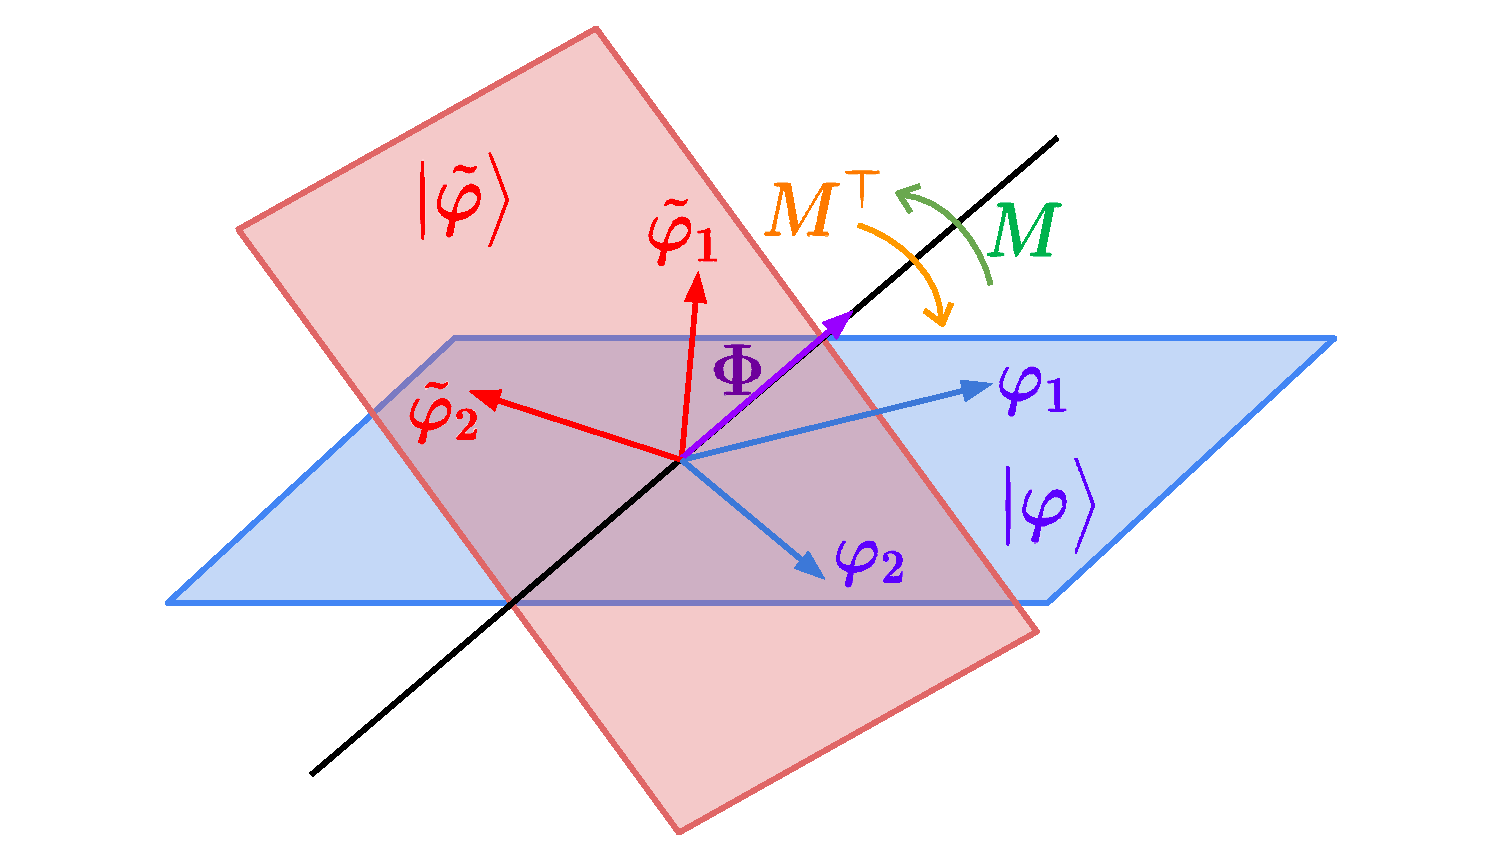
\includegraphics[width=\textwidth]{parts/part1/figures/geometry_solution.pdf}
            \caption{Geometric interpretation of the solution method. The solution vector \( \Phi \) lies at the intersection of two distinct planes, spanned by \( |\varphi\big> \) and \( |\tilde{\varphi}\big> \). The projection matrices \( M \) and \( M^\top \) map vectors between these planes. The eigenvectors of \( MM^\top \) and \( M^\top M \) provide the valid coefficients for the solution in each respective basis.}
        \label{fig:geometry_solution}
    \end{subfigure}%
    \hfill
    % Right Subfigure
    \begin{subfigure}[t]{0.485\textwidth}
        \centering
        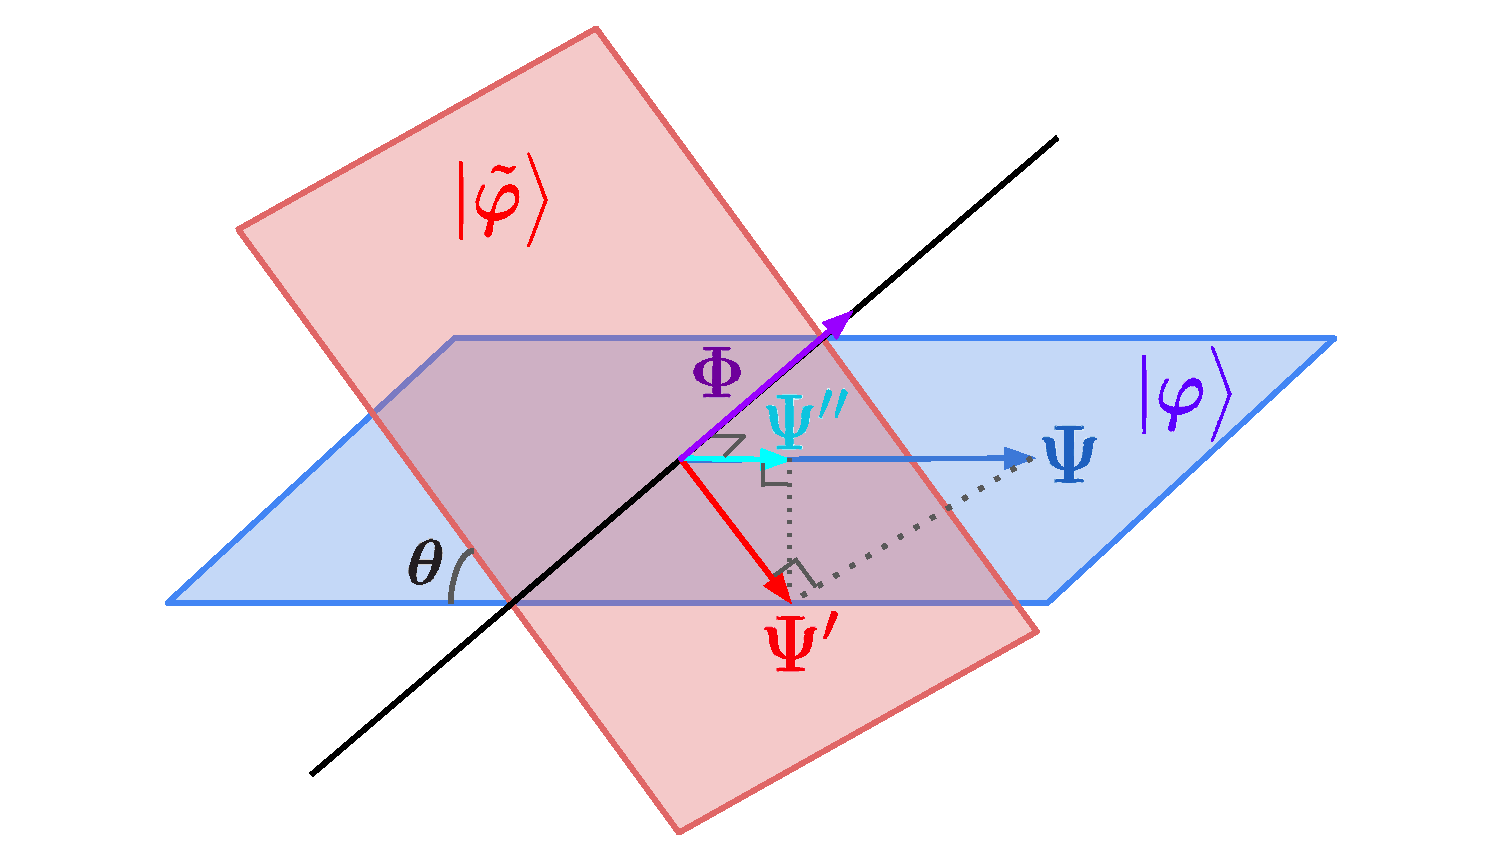
\includegraphics[width=\textwidth]{parts/part1/figures/geometry_non_solution.pdf}
        \caption{Geometric interpretation of the non-solution eigenvector \( \Psi \). Its magnitude is not conserved upon projection back and forth between the planes, resulting in an eigenvalue strictly less than $1$.}
        \label{fig:geometry_non_solution}
    \end{subfigure}
\end{figure}

In this 2D analogy, \( MM^\top \) possesses two eigenvectors, \( \vec{c}_1 \) and \( \vec{c}_2 \), which are orthogonal to one another. Assume $\vec{c}_1$ contains the coefficients that successfully construct the target solution $\Phi$. The second eigenvector, $\vec{c}_2$, constructs a different vector \( \Psi \), which initially lies entirely in the \( |\varphi\big> \) plane (see \cref{fig:geometry_non_solution}). When \( \Psi \) is projected onto the \( |\tilde{\varphi}\big> \) plane, only the component parallel to this new plane survives, yielding \( \Psi' = \cos(\theta) \Psi \), where \( \theta \) is the dihedral angle between the planes. Projecting \( \Psi' \) back onto the original \( |\varphi\big> \) plane produces \( \Psi'' = \cos^2(\theta) \Psi \). While the direction of \( \Psi \) is preserved, its magnitude is attenuated by a factor of \( \cos^2(\theta) \). Consequently, \( \vec{c}_2 \) is an eigenvector of \( MM^\top \) with an eigenvalue of \( \cos^2(\theta) \). As the angle between the planes decreases, the eigenvalue approaches $1$; conversely, if the planes are nearly orthogonal (\( \theta \approx \pi/2 \)), the eigenvalue approaches zero.


Since our goal is to find \( \Phi \), not \( \Psi \), we selectively isolate the eigenvectors of \( MM^\top \) and \( M^\top M \) that are associated with eigenvalues equal to $1$.

This geometric angle between the planes serves as an excellent analogy for the functional difference between the two bases in our wave equation, which is dictated by the parameters \( \mu \) and \( T \). If the mass \( \mu \) decreases and $T \approx N^{\pm1}L$, the discrepancy between the two bases diminishes. Geometrically, the planes become more aligned (smaller $\theta$), yielding a greater number of eigenvalues near $1$. 


\section{Results for the Toy Model}\label{sec:toy_model}

% Structure:
% 1. Details of the problem
% 2. Solution with \mu=0.5, T=\pi, L=2\pi, show the solution, x-t plot, cylinder plot, and the distribution of the coefficients
% 3. varies \mu, show the x-t plot and distribution of the coefficients
% 4. varies T, show the solutions

To ensure the two bases are consistent at high $k$ modes, we require $T = N^{\pm1}L $. For this demonstration, we choose $L=2\pi$ and $T=\pi$, utilizing Neumann initial conditions (ICs) for the perturbations. This ensures that the discrete $k$ values satisfying the spatial BCs are integers, and the solutions are either symmetric or anti-symmetric at both the Bang and the end of the universe, closely mimicking the temporal BCs required for perturbations in a periodic universe \cite{2022PhRvD.105h3514L}. The particle mass is set to $\mu = 0.1$ for the subsequent figures.

\cref{fig:coefficients_T3.14_m0.1} displays the linear combination coefficients for the first four solutions projected onto the basis \(|\phi\big>\). It is evident that each solution inherently requires a superposition of modes with varying frequencies.

\cref{fig:solution_T3.14_m0.1} illustrates the amplitude evolution over time for the four lowest-order solutions, measured at the spatial coordinate $x=\pi$. The time series reconstructed independently from the two bases are visually identical, validating our foundational assumption in \cref{eq:linear_combination} that a valid solution must be a convergent linear combination of both bases.


\begin{figure}
    % Editor's note: Removed the stray closing parenthesis in the caption/text reference for this figure.
    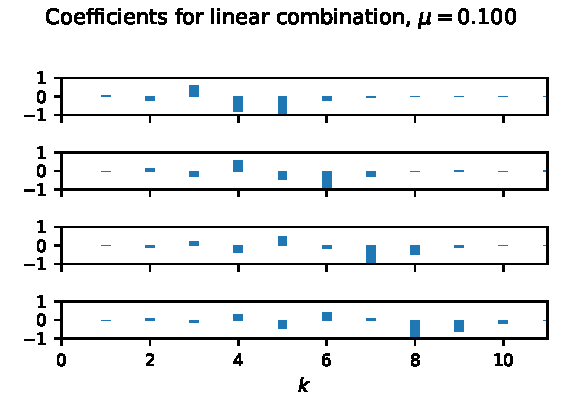
\includegraphics[width=0.7\textwidth]  {parts/part1/figures/eigenvalue_2d_N30_Nt150_T3.14_m0.100_coefficients.pdf}
    \centering
        \caption{The linear combination coefficients of the first four valid solutions, corresponding to the basis $|\phi\big>$, sorted by the frequency of their dominant mode. The coefficients are normalized to a maximum of $1$. The x-axis represents $k \in \mathbb{N}$, which are the strictly allowed wave vectors for the basis $|\phi\big>$.}
        \label{fig:coefficients_T3.14_m0.1}
\end{figure}

\begin{figure}
    % Editor's note: Removed the stray closing parenthesis in the caption/text reference for this figure.
    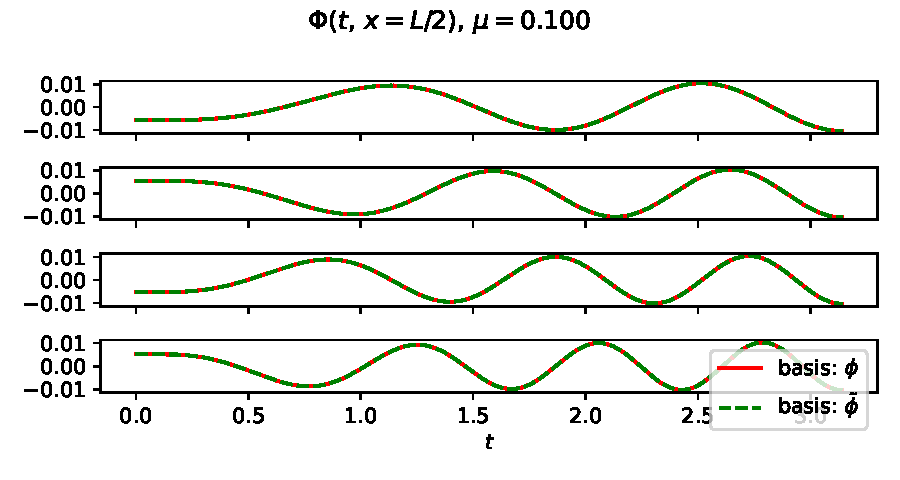
\includegraphics[width=0.8\textwidth]{parts/part1/figures/eigenvalue_2d_N30_Nt150_T3.14_m0.100_xpi.pdf}
    \centering
        \caption{Amplitude-time traces of the numerical solutions evaluated at \(x = \pi\). The red solid lines and the green dashed lines represent the solutions reconstructed using the bases \(|\phi\big>\) and \(|\tilde{\phi}\big>\), respectively.}
        \label{fig:solution_T3.14_m0.1}
\end{figure}


\cref{fig:contour_T3.14_m0.1} presents the corresponding contour plots in the \(x\)-\(t\) plane for these four solutions. The distinctive V-shaped interference patterns arise directly from the superposition of multiple wave frequencies. Specifically, combining simple plane-wave checkerboard patterns (see \cref{fig:plane_waves_x-t_contour}) with different frequencies naturally generates these V-shaped patterns.

\cref{fig:contour_cylinder_T3.14_m0.1} visualizes the solution exhibiting a dominant \(k=5\) mode wrapped onto a cylinder, akin to Fig.~2 in \cite{2021arXiv210906204B}. Here, the azimuthal \(x\)-\(y\) plane represents a closed spatial dimension, while the vertical \(z\)-axis corresponds to conformal time. This visually reinforces that the perturbation perfectly respects periodicity in both space and time.


\begin{figure}[htbp]
    \centering
    % Left Subfigure
    \begin{subfigure}[b]{0.58\textwidth}
        \centering
        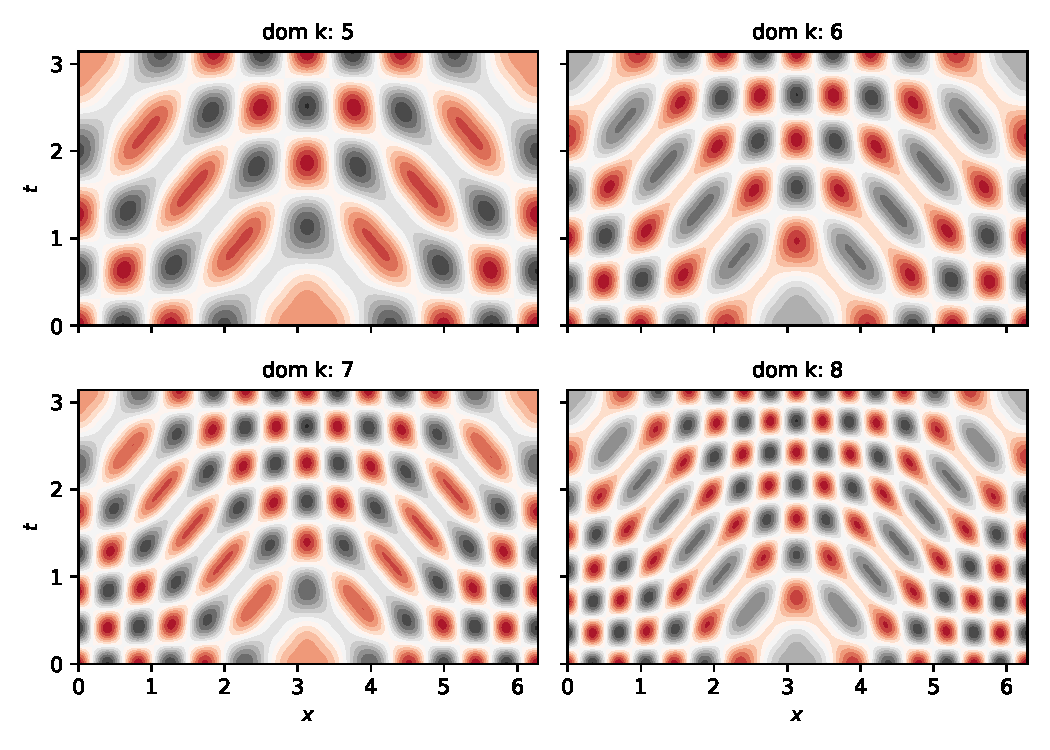
\includegraphics[width=\textwidth]{parts/part1/figures/eigenvalue_2d_N30_Nt150_T3.14_m0.100_contour_sequences.pdf}
        \caption{Spatiotemporal (\(x\)-\(t\)) contour plots for the first four fundamental solutions.}
        \label{fig:contour_T3.14_m0.1}
    \end{subfigure}%
    \hfill
    % Right Subfigure
    \begin{subfigure}[b]{0.39\textwidth}
        \centering
        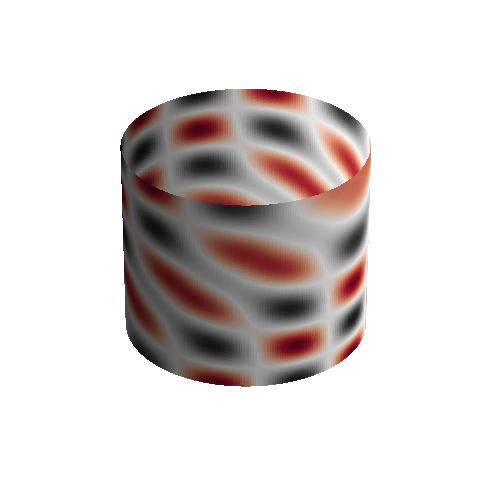
\includegraphics[width=\textwidth]{parts/part1/figures/eigenvalue_2d_N30_Nt150_T3.14_m0.100_cylinder_kdom5.pdf}
        \caption{Cylindrical projection of the solution with a dominant mode of \(k=5\). The azimuthal direction represents the closed spatial dimension, while the vertical axis maps to conformal time.}
        \label{fig:contour_cylinder_T3.14_m0.1}
    \end{subfigure}
\end{figure}

Finally, we consider the impact of varying the particle mass $\mu$. As previously noted, an increase in $\mu$ widens the discrepancy between the two bases, analogous to increasing the dihedral angle between the 2D planes in \cref{fig:geometry_solution}. Consequently, fewer eigenmodes possess eigenvalues sufficiently close to one, leading to an increased number of "missing" or forbidden modes in the low-$k$ regime. \cref{fig:dom_k_vs_m} shows the lowest dominant $k$ as a function of particle mass. It is clear that as the mass increases, the lowest permissible dominant mode is pushed toward larger values of $k$ due to these missing modes. Similarly, as eigenvalue threshold increases, more low-$k$ modes are omitted of their smaller eigenvalues.

\begin{figure}
    % Editor's note: Removed the stray closing parenthesis in the caption/text reference for this figure.
    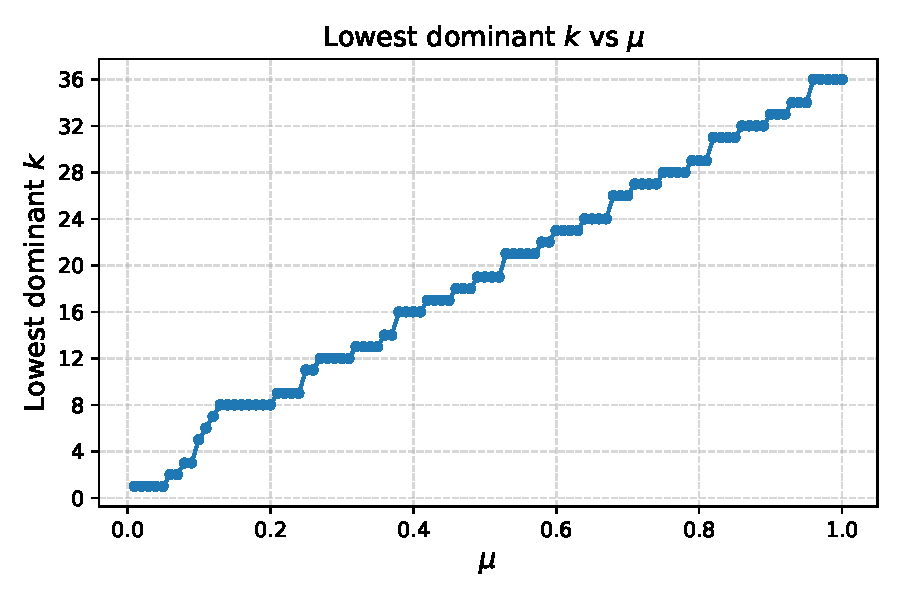
\includegraphics[width=0.7\textwidth]{parts/part1/figures/dom_k_vs_mu.pdf}
    \centering
    \caption{The lowest dominant mode across different particle masses. When mass increase, there would be more missing modes, pushing the lowest dominate $k$ to higher value. }
    \label{fig:dom_k_vs_m}
\end{figure}

\section{Applications to Cosmological Perturbations}\label{sec:real_cosmology_lowk}

We now apply this methodology to a cosmological perturbations. Several physical and numerical complexities must be addressed:

\begin{enumerate}
    \item \textbf{Cosmological Parameters:} Real cosmology introduces several parameters that dictate the expansion history. These parameters must be constrained not only by demanding consistency between the two bases, but also by ensuring alignment with observations.
    \item \textbf{Coupled Fields:} The toy model features only a single scalar field, whereas realistic cosmology requires multiple perturbation fields to be coupled together. A physically valid solution must ensure that all perturbation fields simultaneously match the BCs using a single set of shared linear combination coefficients.
    \item \textbf{Phenomenological Preference:} In the toy model, any arbitrary linear combination of valid eigen-solutions will still satisfy both BCs. However, in cosmology, certain bases (specifically, those approaching pure integer modes) are phenomenologically preferred when comparing predictions to standard observational expectations. 
\end{enumerate}

The strategies utilized to address each of these points are detailed in the following subsections.

\subsection{Determination of Cosmological Parameters}

In the toy Klein-Gordon equation, the sole background parameter is $T$ (time period), which must satisfy $T=N^{\pm 1}\pi$ (where $N\in\mathbb{N}$) to ensure the temporally allowed $k$ modes converge to integers at high-$k$. Similarly, in cosmology, multiple parameters ($\Omega_m, \Omega_K, \Omega_b, h$) must be jointly determined such that the conformal age of the universe satisfies $\eta_{\text{age}}= N^{\pm1}\sqrt{3}\pi$. Furthermore, observational data (e.g., the CMB power spectrum) impose stringent external constraints on these parameters. 

To determine the optimal cosmological parameters satisfying both conditions, we employ a three-step procedure: 
(1) We use a \texttt{KDTree} algorithm to interpolate the CMB likelihood surface $\chi^2(\Omega_m,\Omega_K,\Omega_b,h)$, identifying regions of parameter space that broadly fit observations. This prevents the wasteful execution of expensive ODE solvers on observationally excluded parameters. 
(2) We utilize \texttt{Optuna}, an efficient machine learning optimization framework, to precisely locate the parameter combinations that minimize the deviation of allowed $k$-modes from pure integers. 
(3) From the top 10 best-fit parameter sets, we select the one that yields the lowest $\Delta\chi^2$ against the \texttt{Planck 2018} dataset \footnote{This is achieved by filtering the \texttt{Planck 2018} MCMC samples to isolate those nearest to our candidate parameter sets, and subsequently extracting the corresponding $\Delta\chi^2$ values.}.

% Editor's note: Changed the syntax-breaking \fotnotesize command to a standard font-sizing group to ensure compilation while maintaining intended visual formatting.
{\footnotesize Note that for allowed-$k$ vectors to genuinely map to integers, both their spacing and their intercept must be integers. However, due to lingering theoretical and numerical challenges in obtaining a robust intercept prediction \footnote{To ensure a reliable intercept, our perturbation solver requires two major upgrades: (1) Recombination: The current code directly splices solutions from before and after recombination, rather than integrating continuously through the era. (2) Neutrino physics: Proper modeling requires full neutrino perturbations that transition dynamically from relativistic to non-relativistic states. Both upgrades demand a major rewrite of the perturbation equations and initialization logic.}, the current optimization solely penalizes deviations in the mode spacing, temporarily ignoring the intercept.}

The integer spacing loss function over the cosmological parameter space is illustrated in \cref{fig:loss_param_space}. A lower loss indicates that the allowed-$k$ modes exhibit a spacing closer to exact integers (which is fixed to $4$ in this framework). The red stars indicate our finally selected best-fit parameters: $\Omega_m=0.4445$, $\Omega_K=-0.0394$, $\Omega_b=0.0716$, and $h=0.5615$.

Several physical dependencies are evident in this parameter space. First, the loss function depends heavily on $\Omega_m$ and $\Omega_K$, as these parameters directly dictate the conformal age of the universe. The baryon density $\Omega_b$, plays a more minor role, subtly altering allowed $k$ by shifting the redshift of recombination. \footnote{Since the oscillatory behavior of the perturbations predominantly develops after recombination, altering the recombination redshift primarily shifts the intercept of the allowed $k$-modes. Therefore, tightly constraining $\Omega_b$ will ultimately require restoring the intercept constraint.} Regarding $h$, because the CMB temperature specifically fixes $\Omega_r h^2$, determining the independent values of $\Omega_r$ and $\Omega_\Lambda = 1-\Omega_r-\Omega_m-\Omega_K$ necessary for age calculations inherently requires $h$.

\begin{figure*}
     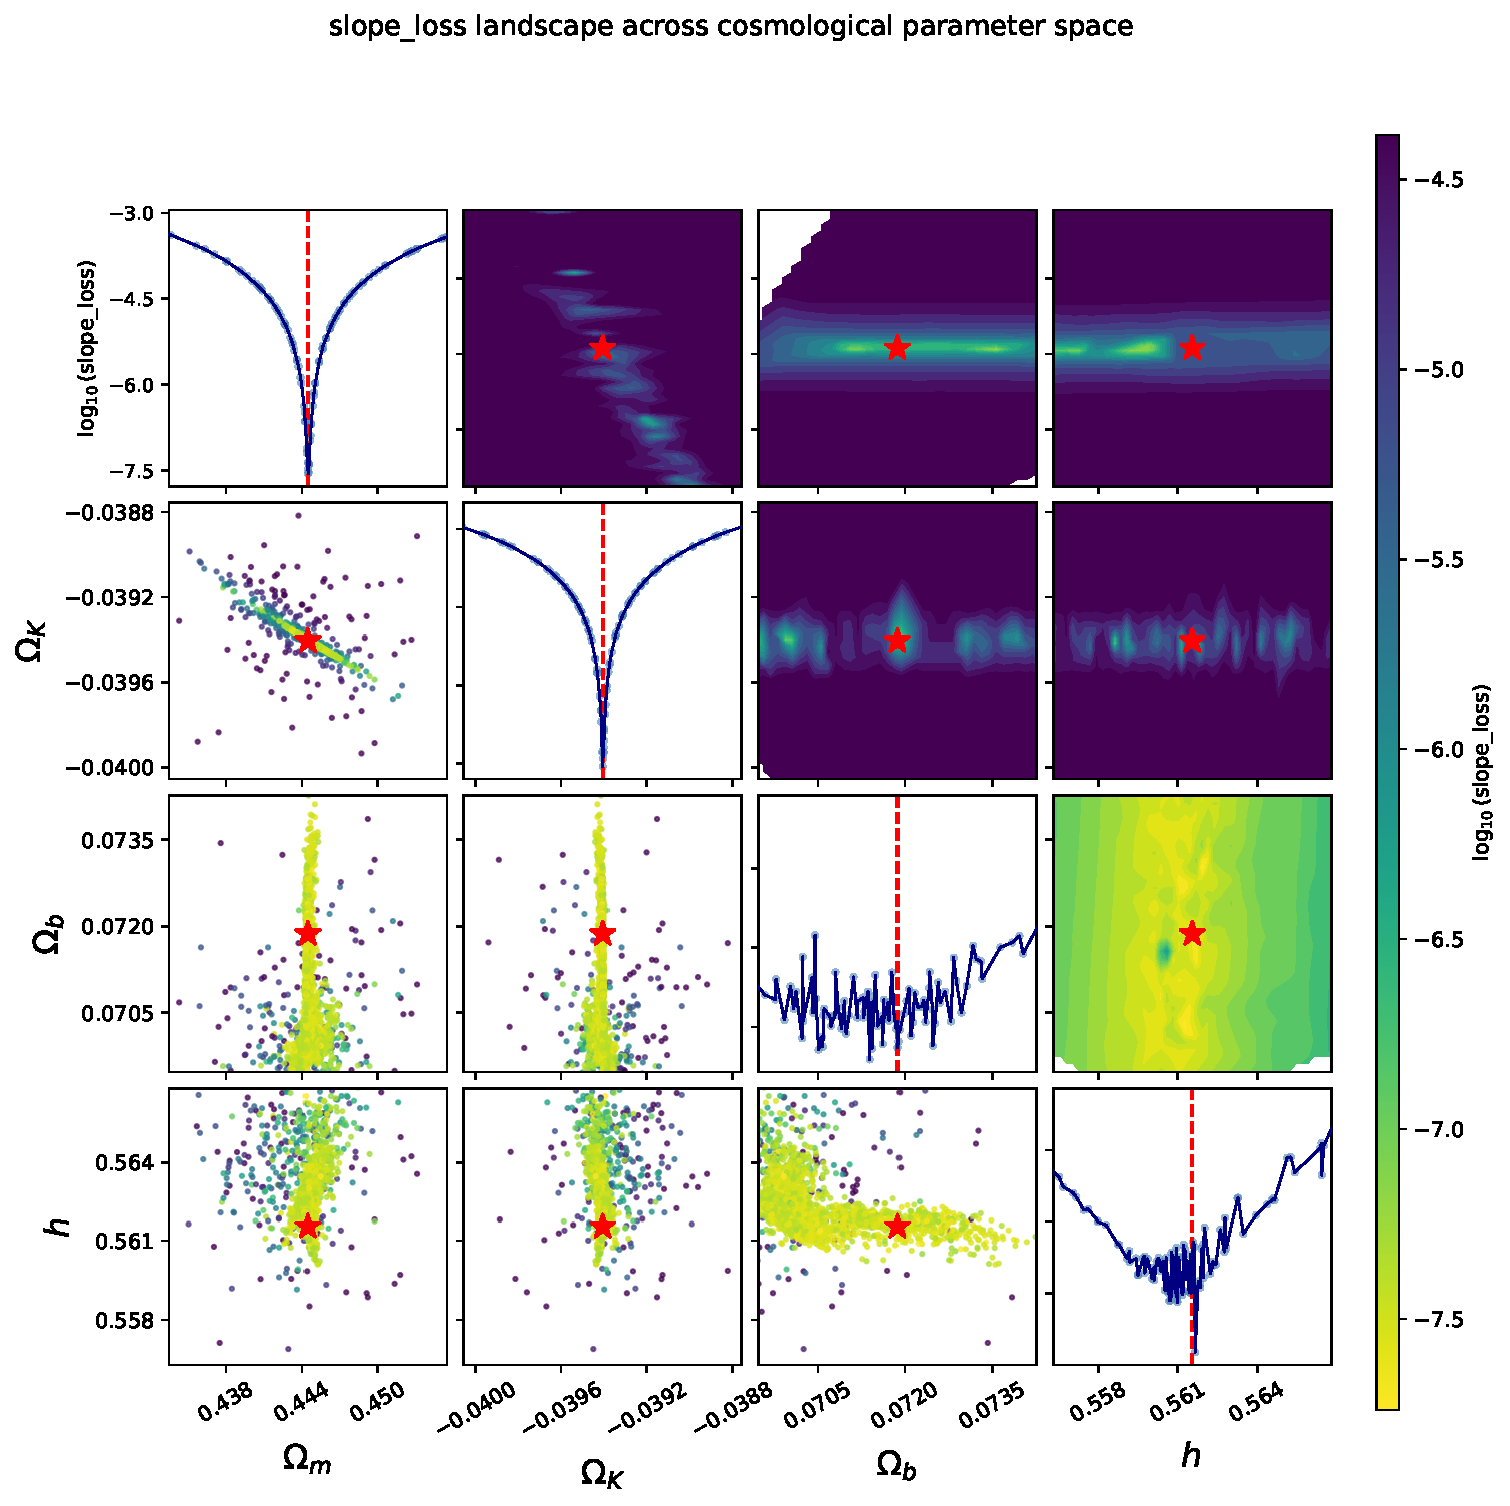
\includegraphics[width=\textwidth]{parts/part1/figures/loss_param_space_Omegab.pdf}
     \caption{The lower triangle contains scatter plots generated by \texttt{Optuna} during the minimization of the integer spacing loss function. The upper triangle displays 2D slices of the loss function where only two parameters are varied, with the others fixed at their best-fit values. The diagonal subplots display the 1D loss functions.}
     \label{fig:loss_param_space}
\end{figure*} 

Finally, we must fix the primordial parameters $A_s, n_s,$ and $\tau$. Because these parameters do not influence the background expansion history, they cannot be constrained by the $k$-spacing requirement. Instead, they govern structure growth and must be fitted directly to observation. We again employ \texttt{Optuna} to find the best-fit $A_s, n_s,$ and $\tau$ by comparing generated spectra to the \texttt{Planck 2018} data. The optimal values yielding the lowest $\Delta\chi^2$ are: $A_s=2.1805\times 10^{-9}$, $n_s=0.9672$, and $\tau=0.0724$. 


\subsection{Coupled Multi-Field Perturbations} 

In a realistic cosmological framework, the evolution involves a minimum of six coupled perturbations: $\Phi, \Psi, \delta_r, \delta_m, v_r, v_m$, supplemented by higher-order Boltzmann moments. To find a single, unified set of linear combination coefficients that simultaneously matches all perturbations across both BCs, the variables must be mathematically concatenated into a single effective field vector: 
\begin{equation}\label{eq:linear_combine_multi_fields}
\begin{aligned}
    \mathbb{X}=\begin{pmatrix}\phi\\\psi\\\delta_r\\\delta_m\\v_r\\v_m \end{pmatrix}, \quad \Phi=\sum_n c_n \mathbb{X}_n=\sum_m c_m \tilde{\mathbb{X}}_m.
\end{aligned}
\end{equation} 
This can also be interpreted as a "stacked" sequential time series, where the effective time coordinate ($\eta$) runs continuously from $0$ to $N\eta_{\text{FCB}}$:
\[ \mathbb{X}(\eta)=\phi(\eta) \oplus \psi(\eta-\eta_{\text{FCB}}) \oplus \delta_r(\eta-2\eta_{\text{FCB}}) \dots\]

Standard linear algebra guarantees that an infinite, complete basis can reconstruct any arbitrary function. In our context, this implies that bases spanning sufficiently high $k$-modes will be able to reliably reconstruct the "stacked" target field, even if hundreds of higher-order Boltzmann terms are strictly included \footnote{In practice, numerically generating bases with a massive number of $k$-modes is computationally prohibitive. Consequently, we limit our current numerical implementation to matching the six primary variables. Nevertheless, the mathematical formalism generalizes natively to include all higher-order terms.}.

\subsection{Phenomenologically Favored Solutions}

To generate the primordial power spectrum (PPS) and CMB power spectrum, phenomenological considerations must be made. Since pure $k\in \mathbb{N}$ modes are conventionally assumed for a closed universe, solutions that most closely resemble isolated integer-$k$ modes are phenomenologically preferred. Analytically, this means we seek a linear combination coefficient matrix $C_{ij}$ that is as sparse as possible, ideally approaching an identity matrix.

With all constraints defined, we search for valid perturbation solutions using \textbf{Canonical Correlation Analysis (CCA)}. CCA normalizes the disparate bases and computes the mutually consistent eigenvectors simultaneously. These global eigen-solutions are then rotated into their sparsest possible representation via an oblique rotation algorithm (\texttt{Promax}), which is specifically designed for non-orthonormal bases. For a rigorous breakdown of the CCA and \texttt{Promax} methodologies, refer to \cref{sec:CCA_sparse}. 

The resulting sparse solutions are shown in \cref{fig:cca_timeseries}. The specific perturbation time series $\delta_r, \delta_m, v_r,$ and $v_m$ generated by the allowed-$k$ basis and the integer-$k$ basis are perfectly aligned, proving that they are valid solutions satisfying both spatial and temporal BCs simultaneously \footnote{Because the metric potentials $\Phi$ and $\Psi$ are strictly determined by $\delta_r, \delta_m, v_r,$ and $v_m$ (via Eq.~6 in \cite{pjz6-47jv}), matching the fluid variables guarantees that the metric variables also match.}. Examining the temporal BC specifically, the density perturbations $\delta_r$ and $\delta_m$ must be symmetric at the Future Big Crunch (FCB). As shown, their temporal derivatives cleanly approach zero at the FCB. Conversely, the velocity perturbations $v_r$ and $v_m$ must be anti-symmetric, and their respective curves correctly cross zero at the FCB.

\begin{figure*}[htbp]
     \centering
     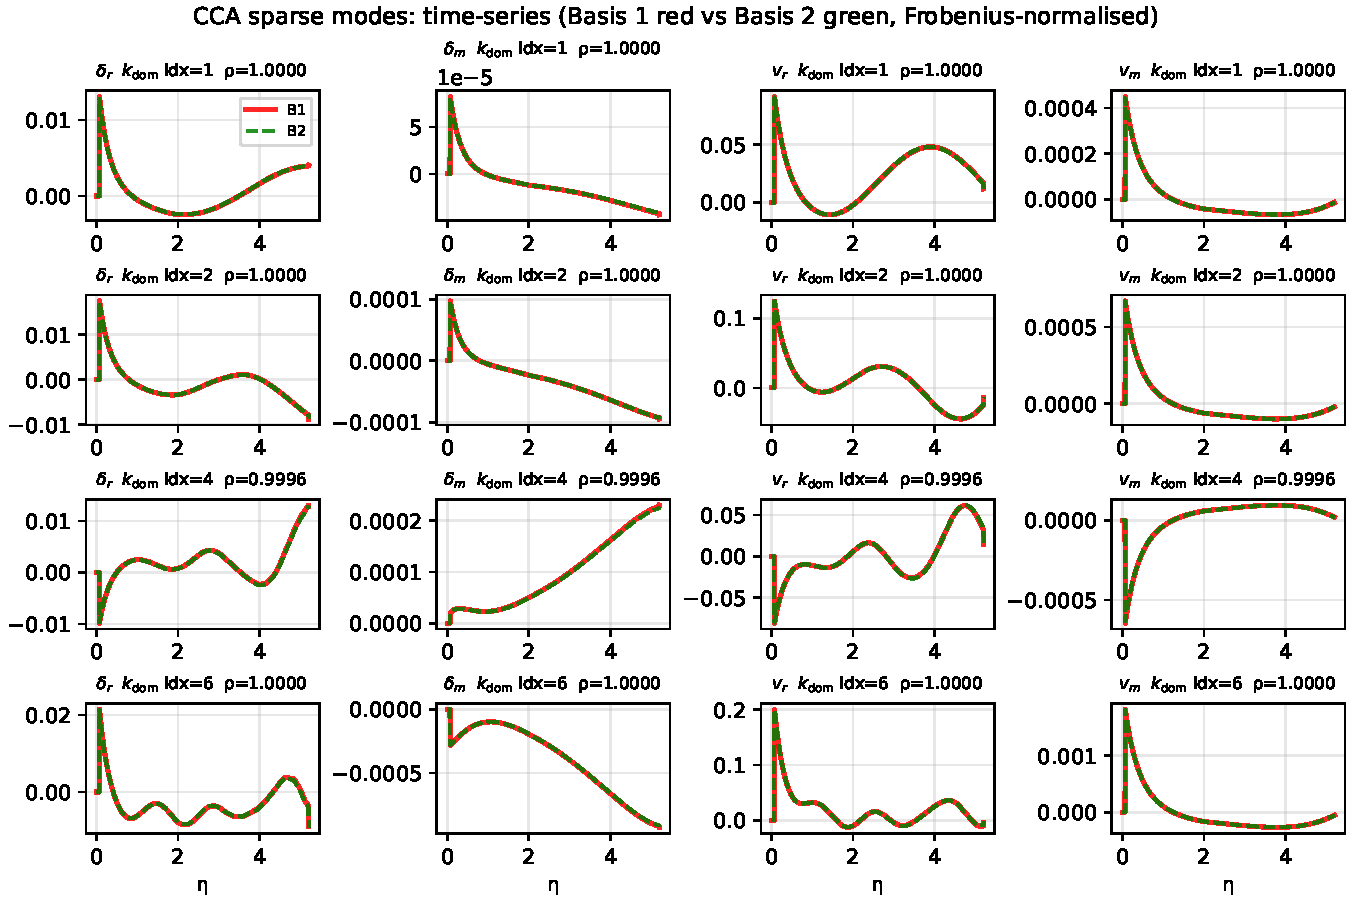
\includegraphics[width=\textwidth]{parts/part1/figures/cca_timeseries.pdf}
     \caption{The first four valid perturbation solutions with the lowest dominant $k$. The time series reconstructed from the allowed-$k$ basis and the integer-$k$ basis overlap exactly, confirming that the solutions successfully satisfy both spatial and temporal boundary conditions.}
     \label{fig:cca_timeseries}
\end{figure*}

% Editor's note: Corrected a broken reference to the figure here (\cref{heatmap_with_delta_k} -> \cref{fig:heatmap_with_delta_k}) based on the label defined in the LaTeX.
\cref{fig:heatmap_with_delta_k} visualizes the coefficient matrix (projected onto the integer-$k$ basis) for the valid sparse solutions. The x-axis represents the available integer-$k$ indices, and each column contains the specific coefficients for a valid composite solution, sorted by its dominant $k$-mode. The lower panel tracks the numerical difference between the temporally allowed $k$-modes and integer-$k$ (defined as allowed-$k$'s nearest integers) \footnote{Because the integer-$k$ sequence is derived by rounding the allowed-$k$ sequence, a sawtooth pattern of residuals naturally emerges. At low $k$, the allowed $k$-spacing is highly non-integer, causing this discrepancy to accumulate rapidly. Once the accumulated difference exceeds $0.5$, the rounding shifts to the next integer, manifesting as a sharp jump in the residual track.}. Where this difference is near zero, the two bases naturally align; the valid solution behaves essentially as a pure mode, and the local coefficient matrix approximates an identity matrix. Conversely, large differences force the CCA to actively mix multiple modes or omit them entirely to maintain consistency. The physical ramifications of this mode mixing and omission on the PPS and CMB are analyzed below.

\begin{figure}[htbp]
     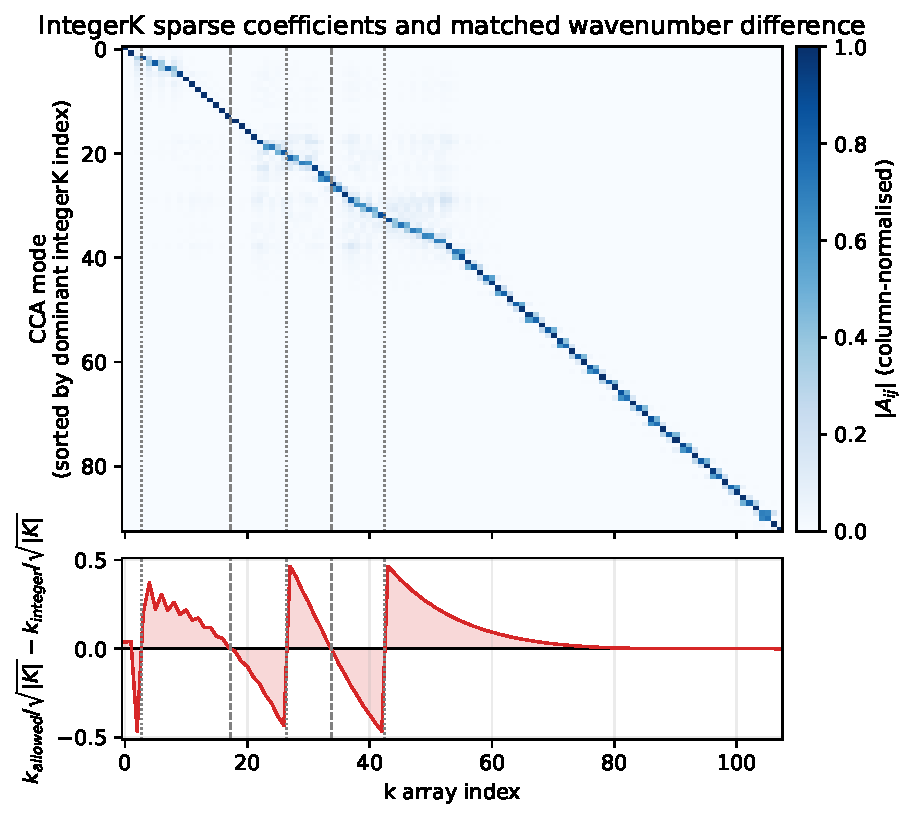
\includegraphics[width=0.8\textwidth]{parts/part1/figures/cca_integerK_heatmap_with_delta_k.pdf}
     \centering
     \caption{Top: Heatmap of the linear combination coefficients for valid sparse solutions. Bottom: The numerical difference between the allowed-$k$ values and the reference integer-$k$ values. Regions of high and low discrepancy are highlighted with dotted and dashed lines, respectively.}
     \label{fig:heatmap_with_delta_k}
\end{figure} 

\section{Generation of Primordial Power Spectra and CMB Spectra}\label{sec:PPS_CMB}

To generate the CMB power spectrum, a fully self-consistent treatment would require extracting the raw perturbation basis directly from a Boltzmann code (e.g., \texttt{CLASS}), executing the CCA to find valid superpositions, and then feeding those exact coupled time-evolutions back into the code to evaluate the true line-of-sight integration internally. However, extensively modifying a standard Boltzmann solver to accommodate this framework is a substantial undertaking that lies beyond the scope of this chapter. (We anticipate that the advancements in large language models may facilitate this complex software engineering task). For the present study, we employ several simplifying assumptions to outline the qualitative effects of this theory on cosmological observables.

In the previous section, we have isolated the sparse valid solutions $\Phi_\lambda$ that satisfy both BCs. Now we use them to construct the PPS and CMB power spectra. The true physical field should be a generalized linear combination of these valid eigenmodes: $\varPhi_{\text{true}}(x) = \sum_\lambda c_\lambda \Phi_\lambda(x)$, where the variance of the coefficients $c_\lambda$ is fundamentally dictated by the PPS.

We hypothesize that the underlying primordial generation mechanism (e.g., inflation) produces an effective spectrum identical to the standard scale-invariant expectation: $P_{std}(k)=A_s(k/k_\star)^{n_s-1}$, where the parameters $A_s$ and $n_s$ are fixed by the early universe physics. Accordingly, the variance of the physical coefficients $c_\lambda$ is assigned as:
\[ \langle |c_\lambda|^2 \rangle =A_s (k_{dom}/k_\star)^{n_s-1}\]
where $k_{dom}$ is the dominant $k$-mode of the specific composite solution $\Phi_\lambda$.

To derive the observable PPS, one must sum the specific fractional contributions across all valid solutions at a given integer $k$:
\begin{equation}
    P_{obs}(k) = \sum_\lambda \langle |c_\lambda|^2 \rangle \times |a_{\lambda k}|^2
\end{equation}
Crucially, $P_{obs}(k)$ naturally reduces to the standard $P_{std}(k)$ in regimes where all valid solutions are pure integer-$k$ modes (i.e., when $a_{\lambda i}=\delta_{\lambda i}$ and $k_{dom}=k$). 

The resulting PPS is presented in \cref{fig:PPS_cca}. We observe a distinct, general power suppression accompanied by severe fluctuations in the low-$k$ region. This is a direct consequence of the omitted and heavily mixed modes necessitated by the boundary mismatches at low $k$ (as mapped in \cref{fig:heatmap_with_delta_k}). Moving to higher frequencies, there is a stable plateau between $k \approx 1.8 \times 10^{-3} \text{ Mpc}^{-1}$ and $3.3\times 10^{-3} \text{ Mpc}^{-1}$, corresponding perfectly to the first identity-matrix region in \cref{fig:heatmap_with_delta_k} where the two bases momentarily synchronize. Finally, at high $k$ ($k > 9\times 10^{-3} \text{ Mpc}^{-1}$), the PPS permanently asymptotes back to the standard scale-invariant model as the asymptotic spacing of the allowed modes converges to integers.
% However, there is lots of wiggling. It is because numerical issue. At high k, the mode completes many oscillations between recombination and the FCB. The phase accumulated is $φ ≈ k·(η_{FCB} − η_{rec})$. A shift of $Δk$ shifts the final phase by $Δφ ≈ Δk·(η_{FCB} − η_{rec})$. Because $Δk$ is small but $(η_{FCB} − η_{rec})$ is large, $Δφ$ can be an arbitrary fraction of $2π$, placing the integerK solution at a completely different phase at the FCB relative to the allowedK solution — hence the shape of perturbations quite different for integerK despite $Δk/k$ being tiny. 

\begin{figure}
     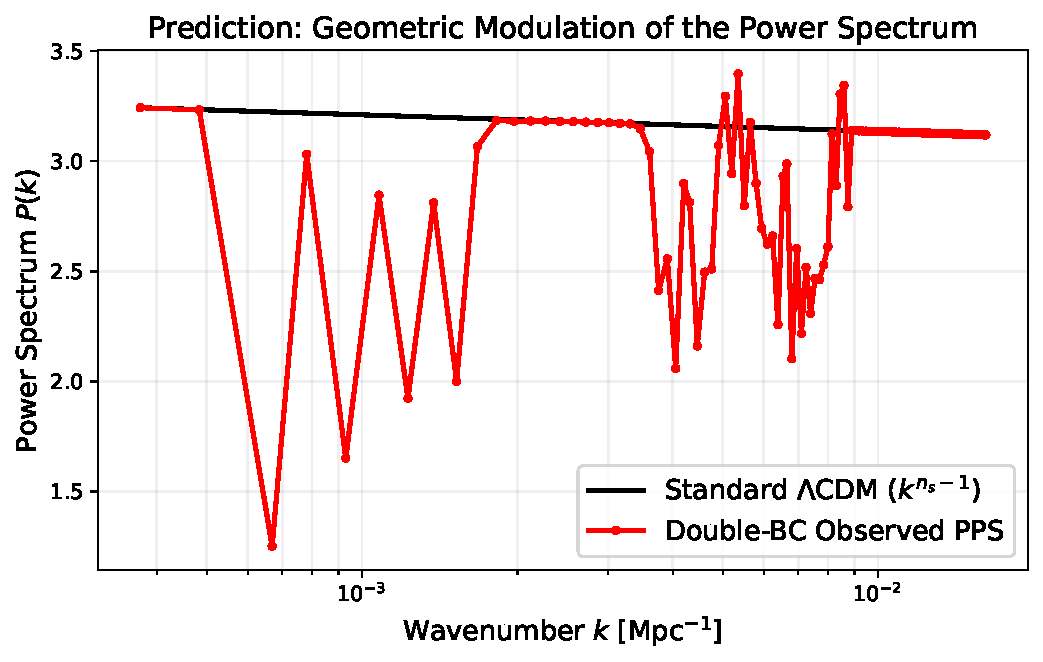
\includegraphics[width=0.75\textwidth]{parts/part1/figures/PPS_power_spectra_cca_2D_dk_penalty_smooth_highK_As_ns_tau_bestfit.pdf}
     \label{fig:PPS_cca}
     \centering
     \caption{The predicted PPS resulting from the valid linear combined solutions. Notably, there is a pronounced suppression and high-variance fluctuation in the low-$k$ regime, which smoothly transitions back to a standard scale-invariant spectrum at high $k$.}
\end{figure} 

Finally, we inject this modified PPS into the Boltzmann solver \texttt{CLASS} to evaluate its impact on the observable CMB temperature power spectrum. The results are plotted in \cref{fig:CMB_cca}. 
% \footnote{$C_\ell^{EE}$ and $C_\ell^{TE}$ are ignored, since the signal are both approach to zero in low $\ell$ mode, making it hard to be distinguished from the standard one}. 
As expected, the suppressions and fluctuations present in the low-$k$ PPS are transferred directly into the low-$\ell$ CMB multipoles. Interestingly, these generic features possess the potential to physically explain longstanding anomalies observed in the \texttt{Planck 2018} dataset \footnote{For instance, the anomalously low quadrupole ($\ell = 2$) relative to the standard $\Lambda\text{CDM}$ theoretical prediction, as well as the higher variance scatter in adjacent low-$\ell$ bins.}. Unfortunately, the inherently large cosmic variance at these scales limits the statistical significance of any such comparison. Because this variance is a fundamental statistical limit arising from having only one observable universe, it cannot be overcome by simply increasing CMB detector resolution. Definitively confirming this model will likely require independent 3D probes of ultra-large-scale structure, such as future galaxy surveys or 21cm intensity mapping arrays, to break this statistical degeneracy.

\begin{figure}
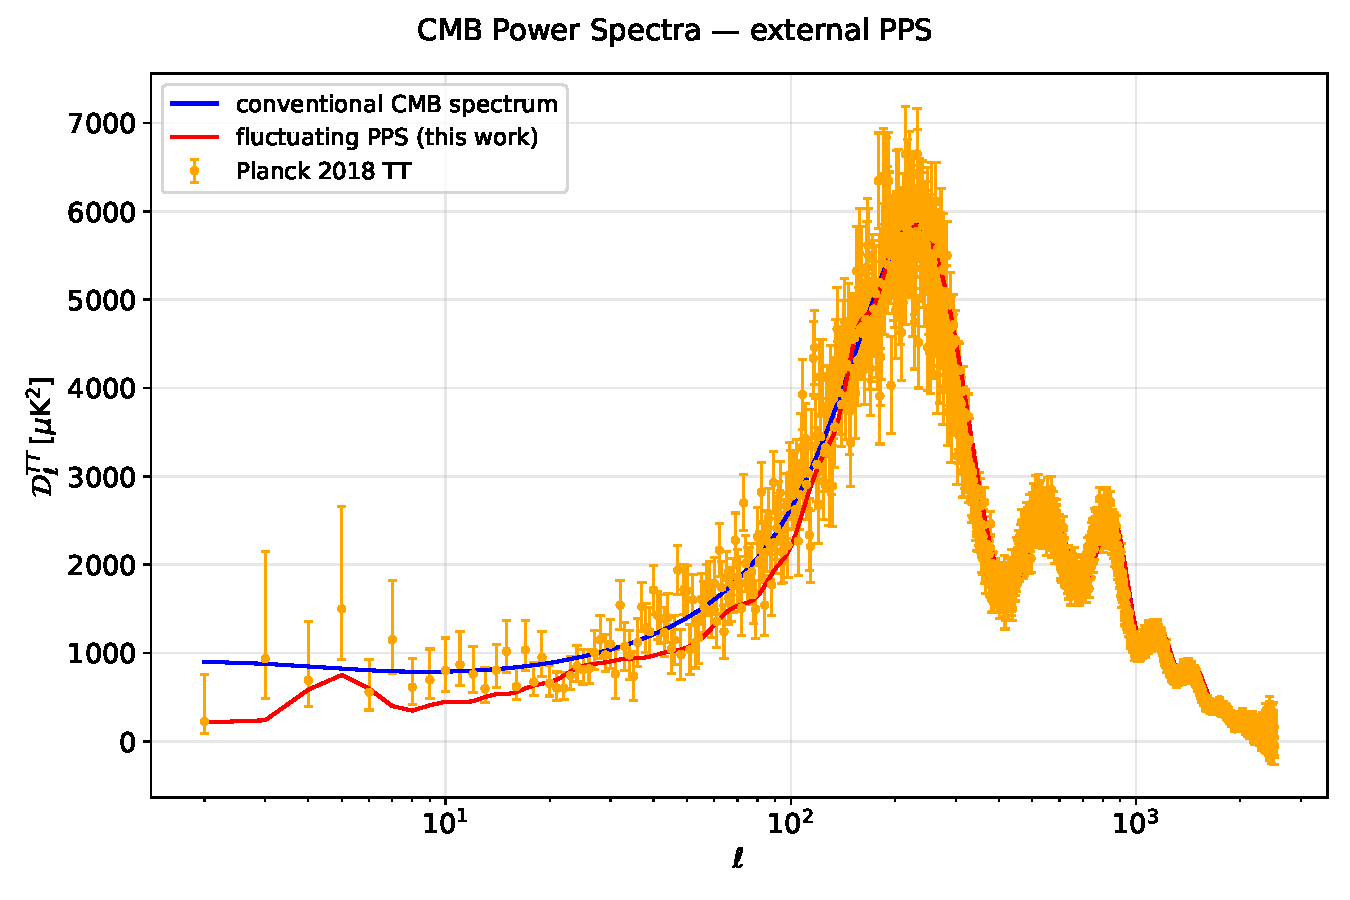
\includegraphics[width=0.9\textwidth]{parts/part1/figures/CMB_TT_externalPPS.pdf}
     \centering
     \caption{The CMB power spectrum generated using our modified PPS. The distinct suppression and fluctuation signatures at low $\ell$ are driven entirely by the constraints imposed by the dual boundary conditions.}
     \label{fig:CMB_cca}
\end{figure} 

Before concluding this analysis, we would like to emphasize again the assumption and simplification utilized in this pipeline. The methodologies for defining "sparse" acceptable solutions and prescribing the generative coefficients $c_\lambda$ rely on numerical and phenomenological assumptions. Furthermore, the modified PPS was externally forced into \texttt{CLASS} to generate the final CMB curves, without directly modifying the Boltzmann code for the theory.  

Due to these simplifications, the exact multipole positions and specific amplitudes of the fluctuations predicted in \cref{fig:CMB_cca} remain approximate. Substantial numerical work is required to elevate this pipeline to a strictly predictive standard. Consequently, this study should be viewed as a pioneering demonstration of the theoretical necessity of these unified solutions, and a qualitative mapping of how imposing dual boundary conditions irrevocably alters the low-$k$ observable universe.


\section{Future Directions}\label{sec:future_work}

This framework offers a novel paradigm for stress-testing fundamental models of the early universe. Alternative theoretical models—such as specific models of cosmic inflation, quantum initial conditions, modified gravity, or loop quantum cosmology—will inherently predict different baseline PPS profiles, coupled perturbation equations, or foundational temporal and spatial boundary constraints. When processed through our dual-BC matching framework, these varying inputs will produce distinct, model-specific valid solution sets and distinct structural mode-mixing matrices. This, in turn, will manifest as highly specific, testable interference features in the observable CMB \footnote{Provided, of course, that the computational simplifications discussed in the previous section are successfully resolved.}.

Beyond the specific spectral fluctuations, one might ask how else this overarching theory could be empirically validated. Since the spectral distortions are strictly localized to the low-$k$ regime, large-scale structures and the CMB remain the primary direct observables. However, the requirement that the allowed $k$-modes approach integer spacing provides a rigid, independent constraint on the background cosmological parameters themselves \cite{pjz6-47jv} \footnote{If the intercept phase of the allowed-$k$ modes can be accurately modeled and included in the loss function, these constraints would become even tighter, particularly for parameters like $\Omega_b$ that subtly govern the phase shifts across recombination.}. If upcoming high-precision surveys independently confirm cosmological parameters that tightly align with the narrow allowed bands predicted by this periodic model, it would represent compelling circumstantial evidence for our model.

Finally, the mathematical methodology developed here for determining valid solutions in systems with competing spatial and temporal boundary conditions has broad applicability across other domains of physics. While temporal boundary conditions appear uniquely exotic in the context of cosmology, they are mathematically ubiquitous in any tightly constrained oscillatory system. For instance, any physical field confined within a finite spatial cavity that is also driven or constrained to oscillate at fixed specific frequencies presents an identical mathematical challenge. Given the coupled PDEs for such a system, our CCA and oblique rotation pipeline provides a generalized toolkit for extracting the non-trivial, physical resonant modes.


\section*{Data Availability Statement}
The source code and data used for generating all figures and results in this study is publicly available in the GitHub repository \cite{code_for_figures_26xx.xxxx} and Zenodo \cite{code_for_figures_26xx}.

\begin{subappendices}

\section{Canonical Correlation Analysis and Sparse Solutions}\label{sec:CCA_sparse}

\subsection{Problem Statement}

A Boltzmann code produces solutions for cosmological perturbation variables \(\Phi,\Psi,\delta_r, \delta_m, v_r, v_m\) (and various higher-order Boltzmann terms) as functions of conformal time $\eta$ and wavenumber $k$. For a given set of $N_k$ wavenumbers, we generate two distinct bases of solutions:

\begin{itemize}
    \item \textbf{Basis 1} (e.g., integer-$k$): defined by matrices $X^p$ of shape $(N_\eta, N_k)$ for each perturbation type $p$,
    \item \textbf{Basis 2} (e.g., allowed-$k$): defined by matrices $\tilde X^p$ of the same shape,
\end{itemize}
where the rows index conformal time and the columns index the independent $k$-modes.

We seek sets of linear combination coefficient vectors such that the composite time evolution constructed using Basis 1 matches the composite time evolution constructed using Basis 2, simultaneously across all required perturbation types. The desired final result is a set of \textit{sparse} coefficient vectors, where each vector is concentrated on one (or very few) $k$-modes, effectively representing the fundamental, physical joint eigenfunctions of the two conflicting bases.


\subsection{Methodology of Canonical Correlation Analysis and Sparsity}
\subsubsection{The Stacked-SVD Approach}

We first rescale the data matrix for each perturbation type in both bases by its respective Frobenius norm, $\|A\|_F = \sqrt{\sum_{ij} A_{ij}^2}$, defining:
\begin{equation}
\bar{X}^p = \frac{X^p}{\|X^p\|_F},\quad \bar{\tilde X}^p = \frac{\tilde X^p}{\|\tilde X^p\|_F}.
\end{equation}
These normalized arrays are then vertically stacked to create a single master state vector:
\begin{equation}
\mathbb{{\bar X}} = \begin{pmatrix}
\bar{X}^{\delta_r} \\
\bar{X}^{\delta_m} \\
\bar{X}^{v_r} \\
\bar{X}^{v_m}
\end{pmatrix}, \quad \mathbb{{\bar {\tilde X}}} = \begin{pmatrix}
\bar{\tilde X}^{\delta_r} \\
\bar{\tilde X}^{\delta_m} \\
\bar{\tilde X}^{v_r} \\
\bar{\tilde X}^{v_m}
\end{pmatrix}.
\end{equation}
Note that the metric potentials $\Phi$ and $\Psi$ are not directly included in the stack, as their dynamics are strictly locked to the fluid variables via the constraint equations. Higher-order Boltzmann moments are also excluded in this specific numerical implementation to control computational overhead (any number of variables can theoretically be added, provided the basis size $N_k$ is correspondingly increased to provide sufficient degrees of freedom). 

This stacking produces unified state matrices of shape $(4N_\eta, N_k)$. While one could technically apply standard SVD to these stacked matrices directly, this formulation obscures the geometric structure of the problem. Stacking is essentially an ad hoc computational trick to collapse a multi-field system into a single matrix, and the Frobenius rescaling represents a specific, non-unique choice for handling the diverse physical dimensions of the variables. For notational simplicity in the following derivations, we will \textbf{drop the bar notation}, but it should be understood that all data matrices are inherently Frobenius-rescaled.

\subsubsection{Formulating Gram Matrices in Momentum Space }

We introduce a set of positive, dimensionless weighting factors $\{w_p\}$ indexed by the perturbation type \footnote{In principle, one could simply set all $w_p=1$. However, because CCA seeks to maximize total covariance, the objective function would otherwise be overwhelmingly dominated by highly oscillatory, high-variance perturbations (e.g., radiation modes). Setting deliberate weights ensures that slower-evolving modes (e.g., $\delta_m$) hold equal footing during the alignment computation.}. We define the $k$-space Gram matrices from the Frobenius-rescaled data as follows:
\begin{equation}
\begin{aligned}
    G_1\equiv G = \sum_p w_p ({X}^p)^\top {X}^p,\\
    G_2\equiv\tilde G = \sum_p w_p (\tilde{X}^p)^\top \tilde{X}^p,\\
    G_{12}\equiv M = \sum_p w_p (X^p)^\top \tilde{X}^p.
\end{aligned}
\end{equation}
Each of these matrices has the shape $(N_k, N_k)$. Because the input data have been normalized, these Gram matrices remain strictly dimensionless regardless of the original physical units of the underlying perturbation fields \footnote{The initial Frobenius rescaling successfully absorbs the per-basis and per-type scale factors, ensuring that $G_{12}$ automatically carries the geometrically correct cross-scaling $(\|X_1^p\|_F \|X_2^p\|_F)^{-1}$ for each term.}.

The matrices $G_\alpha$ (where $\alpha \in \{1,2\}$) strictly encode the inner products between the $k$-modes as measured across all active perturbation types within basis $\alpha$, acting as normalization metric tensors (analogous to the normalization procedure discussed in \cref{sec:linear_combine_solution}). Meanwhile, $G_{12}$ encodes the cross-correlation maps between the two distinct bases, fulfilling the role of the projection matrix $M$ introduced in \cref{sec:linear_combine_solution}.

\subsubsection{Two-Vector Canonical Correlation Analysis}

CCA seeks two linear combination coefficient vectors—$\boldsymbol{c} \in \mathbb{R}^{N_k}$ for Basis 1 and $\boldsymbol{\tilde c} \in \mathbb{R}^{N_k}$ for Basis 2—that maximize the normalized correlation between their resultant time evolutions:
\begin{equation}\label{eq:cca_correlation}
\rho(\boldsymbol{c}, \boldsymbol{\tilde c}) = \frac{\boldsymbol{c}^\top M \boldsymbol{\tilde c}}{\sqrt{\boldsymbol{c}^\top G \boldsymbol{c} \cdot \boldsymbol{\tilde c}^\top \tilde G \boldsymbol{\tilde c}}}.
\end{equation}
The physical intuition here is clear: $\sqrt{G}\boldsymbol{c}$ represents the amplitude of the combined solution reconstructed within the properly normalized Basis 1 metric, and $\sqrt{\tilde G}\boldsymbol{\tilde c}$ represents the same for Basis 2. \cref{eq:cca_correlation} is simply the inner product of these two reconstructed solutions normalized by their respective lengths, which achieves a maximum of $1$ only when the solutions are functionally identical.

This mathematical operation formally mirrors the geometric projection method described conceptually in \cref{sec:linear_combine_solution}, but it powerfully automates the normalization, isolates the translation-invariant solutions, and transforms the eigenvectors back into the original, non-orthogonal basis space in a single integrated step. It is straightforward to prove that $\sqrt{G}$ and $\sqrt{\tilde G}$ act precisely as transformation matrices that map the raw bases into an orthonormal frame. Taking Basis 1 as an example: 
\begin{equation}
\begin{aligned}
    T_{ij}\varphi_i &=\phi_j  \implies  \varphi_i=T_{ij}^{-1}\phi_j\\
    \big< \varphi_i| \varphi_j\big>&=\delta_{ij}  \implies  \big< \phi_k|(T^{-1})^\top_{ki} T_{jl}^{-1}\phi_l\big>=\delta_{ij}\\
    |\phi_m\big>&\big< \phi_k|(T^{-1})^\top_{ki} T_{il}^{-1}|\phi_l\big>\big< \phi_n|=|\phi_m\big>\big< \phi_n|\\
    G_{mk}(T^{-1})^\top_{ki} &T_{il}^{-1}G_{ln}=G_{mn} \implies(T^{-1})^\top_{ki} T_{il}^{-1}\\
    =G_{km}^{-1} &G_{mn}G_{nl}^{-1}=G_{kl}^{-1}  \implies  G_{kl}=T^\top_{ki} T_{il}.
\end{aligned}
\end{equation}

Returning to the maximization of \cref{eq:cca_correlation}, the problem is efficiently solved via Singular Value Decomposition (SVD):
\begin{equation}
G^{-1/2} M \tilde G^{-1/2} = U \Sigma V^\top,
\end{equation}
where $\Sigma = \operatorname{diag}(\sigma_1, \sigma_2, \dots)$ such that $\sigma_1 \ge \sigma_2 \ge \dots \ge 0$. The resulting canonical correlations are $\rho_i = \sigma_i$, and their corresponding coefficient vectors are:
\begin{equation}
\boldsymbol{c}_i = G^{-1/2} \boldsymbol{u}_i,\quad \boldsymbol{\tilde c}_i = \tilde G^{-1/2} \boldsymbol{v}_i,
\end{equation}
where $\boldsymbol{u}_i$ and $\boldsymbol{v}_i$ are the $i$-th columns of $U$ and $V$, respectively. Because $U$ and $V$ are evaluated in the normalized frame, we multiply them by the transformation matrices $G^{-1/2}$ and $\tilde G^{-1/2}$ to pull the coefficients back into the physical frame of the original bases ($\boldsymbol{c}_i$ and $\boldsymbol{\tilde c}_i$).

Equivalently, the left canonical vectors $\boldsymbol{c}_i$ can be extracted directly from the generalized eigenvalue problem:
\begin{equation}
G^{-1/2} M \tilde G^{-1} M^\top G^{-1/2} \boldsymbol{u} = \lambda \boldsymbol{u},
\end{equation}
with eigenvalues $\lambda_i = \sigma_i^2 = \rho_i^2$. Modes with $\rho_i \approx 1$ represent physically valid joint eigenfunctions, while modes with $\rho_i \ll 1$ indicate temporal trajectories that are fundamentally incompatible between the two bases.

\subsubsection{Constructing Sparse Bases via Oblique Rotations}

The raw CCA coefficient vectors $\boldsymbol{c}_i$ and $\boldsymbol{\tilde c}_i$ are rarely sparse; they emerge as dense, global linear combinations of many $k$-modes because the solver optimizes purely for correlation with no regard for localization. To recover a physically meaningful basis, we seek an invertible rotation matrix $R \in \mathbb{R}^{m \times m}$ such that the rotated coefficient vectors:
\begin{equation}
\begin{aligned}
    &{\boldsymbol{c}}^R_j = \sum_{i=1}^m R_{ji} \boldsymbol{c}_i, \quad \text{i.e.} \\ {C}^R = C R^\top, &\quad C = [\boldsymbol{c}_1 \mid \cdots \mid \boldsymbol{c}_m] \in \mathbb{R}^{N_k \times m},
\end{aligned}
\end{equation}
become optimally sparse (i.e., tightly concentrated on a single $k$-mode or a small cluster of modes). Notably, we do not require the final rotated vectors ${\boldsymbol{c}}^R_j$ to be orthogonal—only sparse.

A common algorithm for this task is \texttt{Varimax} rotation, which rigidly rotates the sub-space frame to maximize the sum of the variances of the squared loadings. However, \texttt{Varimax} strictly enforces orthogonality, preserving the angles between all vectors during the rotation. Because our physical CCA vectors $\boldsymbol{c}^R_i$ are not fundamentally orthonormal in $k$-space, applying rigid \texttt{Varimax} produces severe alignment errors.

To overcome this, we utilize Oblque rotation method \texttt{Promax}, which generalizes \texttt{Varimax} by actively relaxing the orthogonality constraint. It searches for an invertible matrix $R$ (which need not be orthogonal) that refines the \texttt{Varimax} approximation into a form displaying "simple structure" (maximal sparsity). The additional degrees of freedom allowed by non-orthogonal deformation grant \texttt{Promax} the flexibility needed to find a significantly sparser, and therefore more physical, solution than any strictly orthogonal rotation algorithm. 

% \begin{table}[t]
% \centering
% \begin{minipage}{0.8\textwidth}
% \noindent \hrule \vspace{1em}
% \noindent \textbf{CCA-based sparse joint eigenfunction method}  \\ \vspace{0.5em}
% \noindent \hrule \vspace{1em}
% \noindent \textbf{Input:} $X^p, \tilde X^p \in \mathbb{R}^{N_\eta \times N_k}$ for each perturbation type $p$; weights $\{w_p\}$; correlation threshold $\rho_{\min}=0.99$ \\[0.5em]
% \noindent\begin{tabular*}{\textwidth}{@{}r@{\hspace{0.5em}}l@{\extracolsep{\fill}}r@{}}
% 1: & \textbf{Frobenius rescaling}  \\
% 2: & \quad $\bar{X}^p \leftarrow X^p/\|X^p\|_F$ for all $p$, similarly for $\bar{\tilde X}^p$ & \\[0.5em]
% 3: & \textbf{Compute Gram matrices}   \\
% 4: & \quad $G \leftarrow \sum_p w_p ({X}^p)^\top {X}^p$ \\
% 5: & \quad $\tilde G \leftarrow \sum_p w_p (\tilde{X}^p)^\top \tilde{X}^p$ & \\
% 6: & \quad $M \leftarrow \sum_p w_p ({X}^p)^\top \tilde{X}^p$ & \\[0.5em]
% 7: & \textbf{Solve CCA}  \\
% 8: & \quad $U \Sigma V^\top \leftarrow \text{SVD}(G^{-1/2} M \tilde G^{-1/2})$ & \\
% 9: & \quad Keep $m$ components with $\sigma_i > \rho_{\min}$ & \\
% 10: & \quad $\boldsymbol{c}_i \leftarrow G^{-1/2} \boldsymbol{u}_i$ for $i=1,\dots,m$ & \\ &$\triangleright$ Basis 1 $k$-space coefficients \\
% 11: & \quad $\boldsymbol{\tilde c}_i \leftarrow \tilde G^{-1/2} \boldsymbol{v}_i$ for $i=1,\dots,m$ & \\ &$\triangleright$ Basis 2 $k$-space coefficients \\[0.5em]
% 12: & \textbf{Oblique rotation for sparsity} \\
% 13: & \quad $C \leftarrow [\boldsymbol{c}_1 \mid \cdots \mid \boldsymbol{c}_m]$  \\
% 14: & \quad ${C}^R \leftarrow \text{Promax}(C)$ \\
% \end{tabular*} \\[0.5em]
% \noindent \textbf{Output:} $C^R \in \mathbb{R}^{N_k \times m}$ \\
% \hspace*{1.5em} Each column: sparse coefficient vector for a valid joint eigenfunction \\
% % \hspace*{1.5em} For modes with $\rho \approx 1$: $\boldsymbol{c}_i \approx \boldsymbol{\tilde c}_i$ (same coefficients in both bases) \\[0.3em]
% \hspace*{1.5em}
% \noindent \hrule
% \end{minipage}
% \end{table}

\end{subappendices}

\printbibliography[heading=subbibintoc, title={References for Chapter \thechapter}]